\documentclass[12pt]{article}

\usepackage{sbc-template}
\usepackage{graphicx,url}
\usepackage[utf8]{inputenc}
\usepackage[brazil]{babel}
% \usepackage[latin1]{inputenc}

\usepackage[dvipsnames]{xcolor}
\usepackage[normalem]{ulem}
\usepackage{amsmath}

\newcommand{\matheus}[1]{\textcolor{purple}{#1}}
\newcommand{\cmatheus}[2]{\textcolor{purple} {#2}}
\newcommand{\omatheus}[1]{\text{\sout{\matheus{#1}}}}

\newcommand{\daniel}[1]{\textcolor{blue} {#1}}
\newcommand{\cdaniel}[2]{\textcolor{blue} {#2}}
\newcommand{\odaniel}[1]{\text{\sout{\daniel{#1}}}}

\newcommand{\todo}[1]{\textcolor{red}{[ToDo:{#1}]}}

%\newcommand{\cred}[1]{\textcolor{red}{#1}}
%\newcommand{\cblue}[1]{\textcolor{blue}{#1}}

     
\sloppy

\title{Detecção de conflitos diretos em redes IoT utilizando o Maude\footnote{O presente trabalho foi realizado com apoio do Conselho Nacional de Desenvolvimento Científico e Tecnológico (CNPq) - UNIVERSAL 423212/2021-4}}

\author{Matheus de A. M. Pereira\inst{1}, Daniel Ventura\inst{1}}

\address{Instituto de Informática\\
  Universidade Federal de Goiás (UFG) -- Goiânia, GO -- Brazil
  \email{matheus.marpereira@gmail.com, ventura@ufg.br}
}

\begin{document} 

\maketitle

\begin{abstract}
  In this work we explore the conflict detection in distributed networks problem. We propose a logical concurrency model for the network and specify it in the Maude system, which will be able to simulate the network and detect possible conflicts.
\end{abstract}
     
\begin{resumo} 
  Neste trabalho exploramos o problema de detecção de conflitos em redes distribuídas utilizando lógica de reescrita. Propomos um modelo lógico e concorrente para a rede e realizamos a sua especificação no software Maude, que será utilizado para simular a rede e detectar possíveis problemas.
\end{resumo}

\section{Introdução} \label{sec:chap1}

Sistemas IoT são cada vez mais utilizados no mundo, para diversas finalidades como casas inteligentes ou até mesmo cidades inteligentes, com dispositivos conectados remotamente e que conseguem medir e gerenciar algum aspecto do seu ambiente \cite{ConflictDetectionSurvey}. Estes dispositivos podem ser controlados remotamente por algum aplicativo, ou configurados para agirem automaticamente baseado em certos gatilhos.

Montar uma rede IoT pode ser um grande desafio, pois há aspectos importantes que devem ser considerados para garantir que os dispositivos estão agindo corretamente, que as regras configuradas garantam a integridade e a segurança do sistema \cite{ConflictDetectionFuture}.

Este trabalho apresenta uma modelagem para detecção de conflitos em redes distribuídas utilizando o Maude, um framework de Lógica de Reescrita de alta performance. A seção 2 deste trabalho contém uma introdução à Lógica de Reescrita e ao Maude. A seção 3 contém uma descrição do modelo da nossa rede e seus componentes. A seção 4 contém uma breve descrição para o nosso caso de estudo. A seção 5 explica como foi realizada a especificação no Maude. A seção 6 contém os resultados do nosso trabalho e possíveis trabalhos futuros. A seção 7 contém a nossa conclusão sobre este trabalho.

A especificação completa do modelo no Maude pode ser encontrada no endereço: \texttt{https://github.com/mathamp/conflict-detection-maude}.
\section{Lógica de Reescrita} \label{sec:chap2}

Lógica de reescrita é definida como uma \textit{teoria de reescrita sortida} $\mathcal{R} = (\Sigma, E \cup B, R)$, onde $\Sigma$ é a sintaxe com \emph{sorts} da nossa teoria, $E$ é um conjunto de equações terminante e confluente, $B$ um conjunto de axiomas (e.g. associatividade, comutatividade e identidade) e $R$ é um conjunto de regras de reescrita no formato $t \rightarrow t'$ ou no formato condicional: $t \rightarrow t' \texttt{ se } \textbf{condição}$ \cite{RewritingLogicTwentyYears}. Assim, na representação de um sistema computacional utilizando a lógica de reescrita $\mathcal{R}$, a teoria equacional $(\Sigma, E \cup B)$ representa os estados do sistema como tipos de dados algébricos enquanto o conjunto de regras de reescrita $R$ (possivelmente não-confluente) especifica a dinâmica do sistema.

Devido a natureza não-determinística das regras de reescrita, onde qualquer regra de reescrita compatível com um determinado estado do sistema pode ser aplicada, sistemas concorrentes podem ser naturalmente modelados, devido a incerteza sobre a ordem de execução e comunicação entre os dispositivos. 
Por exemplo, considere um quarto com dispositivos inteligentes configurados para ligar o aquecedor quando a temperatura do quarto atingir 10ºC e ligar as luzes quando o horário for 18:30, e que, exatamente às 18:30 a temperatura chegou a 10ºC. Devido a natureza concorrente dos dispositivos, não é possível determinar qual ação ocorrerá primeiro: ligar as luzes ou ligar o aquecedor, mas é possível deduzir os cenários que podem ocorrer como um diagrama de transições:

\begin{figure}[h]
  \centering
  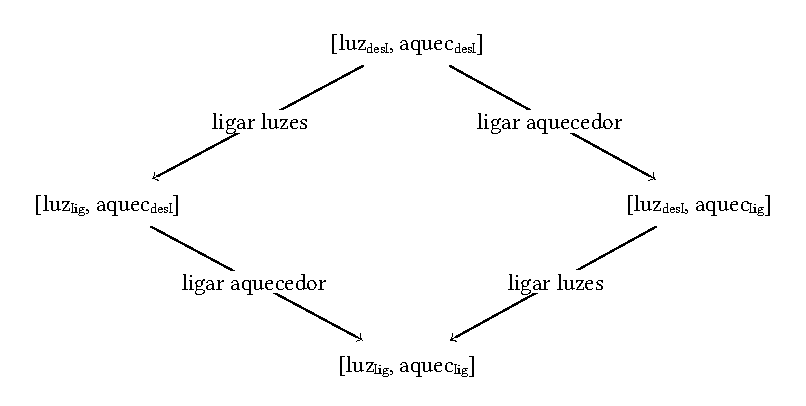
\includegraphics{img/diagram.pdf}
  \caption{Diagrama de transições}
  \label{fig:fig1}
\end{figure}

Este é um exemplo de situação confluente, onde todas as possibilidades de transições convergem para um mesmo estado, mas também existem situações não-confluentes, onde a ordem das transições pode resultar em estados divergentes.

\subsection{Maude} \label{sec:chap2sub1}

O software utilizado para a especificação do nosso modelo será o Maude, um framework em Lógica de Reescrita de alta performance.
No Maude, a sintaxe $\Sigma$ para construir sorts e operadores é definida utilizando o comando \texttt{op}, as equações $E$ utilizando o comando \texttt{eq}, e os axiomas $B$ são definidos entre colchetes como parâmetros no momento da declaração de um construtor.
O par $(\Sigma, E \cup B)$ no Maude deve definir funções totais, podendo serem vistas como programas funcionais.

Abaixo apresentamos uma definição de conjuntos de naturais no Maude para introduzir a sua sintaxe:

\begin{verbatim}
protecting NAT .
sort NatSet .
subsort Nat < NatSet .
\end{verbatim}

\noindent
Primeiro importamos um módulo do prelúdio, chamado \texttt{NAT}, que contém a definição dos números naturais. \\
Definimos um sort chamado \texttt{NatSet} e especificamos que todo \texttt{Nat} também é um \texttt{NatSet}.

\begin{verbatim}
op empty : -> NatSet [ctor].
op _,_ : NatSet NatSet -> NatSet 
            [ctor assoc comm id: empty] .
\end{verbatim}

\noindent
Definimos um construtor de um \texttt{NatSet}, através de uma constante chamada \texttt{empty}. \\
Um construtor infixo posicional também é definido, que precisa de dois sorts \texttt{NatSet} para ser construído, onde \texttt{\_} indica as posições desses sorts no construtor. Também é definido os axiomas de associatividade, comutatividade e \texttt{empty} como identidade para este construtor.

\begin{verbatim}
var N : Nat .
var S : NatSet .

eq N,N = N .

op _in_ : Nat NatSet -> Bool .
eq N in (N,S) = true .
eq N in S = false [owise] .
\end{verbatim}

\noindent
Aqui definimos variáveis para utilizarmos nas nossas equações e operações. \\
A primeira equação traz a propriedade de idempotência para o segundo construtor (Por limitações técnicas, o Maude não consegue lidar com os axiomas \texttt{assoc} e \texttt{idem} juntos). \\
Definimos uma operação para verificar se um elemento está num conjunto através de 2 equações parciais. A primeira equação utiliza \textit{pattern matching} para verificar se o elemento desejado está no conjunto, caso contrário, a segunda equação é utilizada.

Uma especificação no Maude pode ser dividida em módulos, estamos interessados em 2 tipos de módulos específicos:
\begin{itemize}
  \item \textbf{Módulos funcionais:} Permite a definição de teorias equacionais. Será utilizado para especificar os \textit{sorts} que definem a nossa rede, e algumas funções auxiliares.
  \item \textbf{Módulos de sistema:} Permite a definição de regras de reescrita. Será utilizado para especificar a comunicação entre os dispositivos da rede.
\end{itemize}

\noindent
Após especificado o formato da rede e a comunicação entre os dispositivos, uma rede pode ser instanciada e o Maude pode iniciar a busca por estados que representam o acontecimento de conflitos utilizando as regras de reescrita. No Maude, estamos interessados no uso de 2 comandos para a execução das regras de reescrita:
\begin{itemize}
  \item \texttt{rewrite <REDE> .}: Irá aplicar as regras de reescrita de forma determinística. Usado inicialmente para analisar como o Maude está realizando as regras de reescrita e se existem problemas na nossa especificação.
  \item \texttt{search <REDE> =>* <CONFLITO> .}: Verificar se existe alguma ordem de aplicação de regras de reescrita que chega num conflito. Irá explorar todas as possibilidades para aplicação de regras de reescrita, gerando um grafo de busca de estados, que será explorado utilizando uma estratégia de busca em largura. Um detalhe importante no qual deve-se tomar cuidado é não deixar o número de estados crescer subitamente, pois isso impedirá fazer buscas mais profundas em um tempo razoável utilizando o Maude. Note que o crescimento da árvore de busca será determinado pelo número de regras de reescrita aplicáveis em cada estado.
\end{itemize}
\section{Modelo para redes IoT} \label{sec:chap3}

O modelo é baseado na abordagem proposta por %\matheus{(repetição da palavra 'modelo', eu não sei uma maneira melhor de melhorar esta frase)} 
\cite{IoTC2}. A rede IoT consiste de diversos componentes conectados, que comunicam entre si transmitindo eventos, ações e comandos. Entre esses componentes estão: sensores, controladores, atuadores e os dispositivos IoT.

A forma de comunicação entre esses componentes funciona num modelo ``gatilho e ação'': cada dispositivo tem um conjunto de gatilhos, quando um gatilho ocorre, este realizará alguma ação. Sensores medem algum parâmetro do ambiente, e quando este atinge algum limiar, o sensor dispara eventos. Controladores escutam por eventos, e podem disparar ações em resposta. Atuadores escutam por ações, e podem disparar comandos em resposta. É importante ressaltar que um sensor pode emitir eventos para vários controladores, controladores podem receber eventos de vários sensores e emitir ações para vários atuadores, e atuadores podem receber ações de vários controladores. Conforme a quantidade de componentes na rede cresce, é possível que haja sobreposições na comunicação entre os componentes, e isto aumenta as chances de ocorrer conflitos.

\subsection{Configurações e regras} \label{sec:chap3sub1}

Uma rede IoT é montada com a finalidade de atender algum objetivo, por exemplo, ``Manter a temperatura do quarto agradável'', estas são chamadas \textit{regras de ambiente} e devem ser mantidas a todo momento. Se a rede permitir que essas regras sejam quebradas, temos um \textit{conflito de regra de ambiente}.

Os dispositivos da rede podem ser configurados por regras operacionais que ditam o seu comportamento. Um sensor pode ser configurado para observar algum parâmetro da rede e emitir eventos caso o parâmetro observado atinja algum limiar desejado, como por exemplo, ``Se a temperatura chegar em 30ºC, emitir o evento \textbf{Temperatura Quente}''. Um controlador pode ser configurado para escutar por eventos e emitir ações, como por exemplo, ``Ao receber o evento \textbf{Temperatura Quente}, emitir a ação \textbf{Ligar o ar condicionado}''. Um atuador pode ser configurado para escutar por ações e emitir comandos, como por exemplo, ``Ao receber a ação \textbf{Ligar o ar condicionado}, emitir o comando \textbf{Ligar} para o ar condicionado''.

Dependendo de como a rede for configurada, é possível que um atuador receba 2 ações contraditórias ao mesmo tempo, devido a componentes diferentes que estão configurados para atender objetivos diferentes. Por exemplo, um grupo de componentes está configurados para ligar as luzes do quarto enquanto houver pessoas no quarto, enquanto outro grupo de componentes está configurados para desligar as luzes caso esteja de madrugada. Quando houver pessoas na sala de madrugada, as ações \textbf{Ligar luzes} e \textbf{Desligar luzes} serão emitidas, que contradizem entre si. Este tipo de conflito foi identificado como \textit{conflito direto} \cite{ConflictDetectionORAN}.
Conflitos de regra de ambiente também são conflitos diretos.
\section{Caso para estudo} \label{sec:chap4}

Consideramos um quarto com alguns dispositivos IoT para controlar automaticamente sua temperatura e iluminação. Para isso foi configurado um conjunto de sensores, controladores e atuadores para o ar condicionado, o aquecedor e as luzes do quarto.
A rede foi configurada de forma para ligar e desligar automaticamente o ar condicionado ou o aquecedor quando a temperatura estiver muito quente ou fria, e desligá-los quando a temperatura estiver amena. As luzes ligam e desligam automaticamente baseadas na luminosidade do quarto, e ficam desligadas durante a madrugada.
A figura \ref{fig:fig2} mostra um diagrama que representa como os componentes estão conectados.
Para mais detalhes, veja o Apêndice \ref{apx:apx1}.

\begin{figure}[ht]
  \centering
  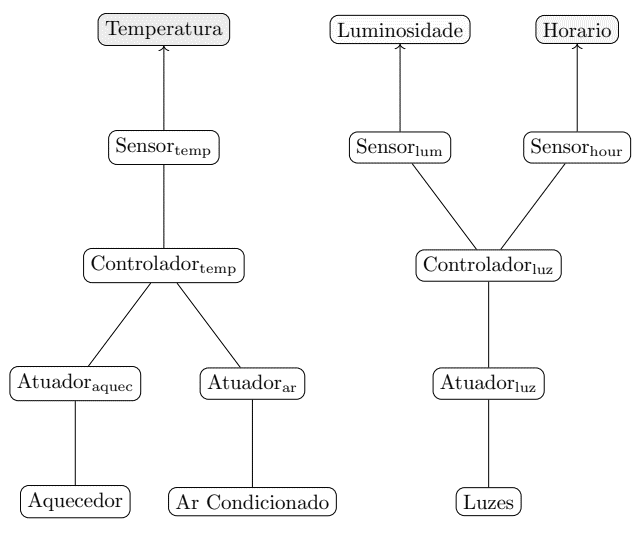
\includegraphics[width=0.5\textwidth]{img/network-diagram.png}
  \caption{Diagrama de componentes}
  \label{fig:fig2}
\end{figure}
\section{Especificação no Maude} \label{sec:chap5}

O ambiente é formado por variáveis de ambiente (temperatura, luminosidade, horário) e componentes (sensores, controladores e atuadores). Os componentes são conectados por canais e escutam por eventos, ações e comandos transmitidos por estes. Estes componentes foram modelados utilizando uma sintaxe definida no Maude. A comunicação entre componentes foram modeladas utilizando regras de reescrita.

Devido a forma que o Maude faz as suas buscas (busca em largura), foi necessário realizar algumas alterações na nossa especificação. Se for permitido que diversas regras de reescrita ocorram \cdaniel{em diversos momentos}{a todo momento}, o grafo de busca irá crescer de forma exponencial.
\cdaniel{No modelo original, não haviam restrições na aplicação das regras de reescrita, o que frequentemente faria o Maude explorar cenários indesejadas de evolução da rede. Por exemplo, um dispositivo poderia ficar reemitindo a mesma ação diversas vezes, embora isto possa ser um cenário real, isto prejudica a busca do Maude, aumentando consideravelmente o grafo de estados.}{Não haviam restrições na aplicação das regras de reescrita no modelo original, frequentemente gerando cenários irrelevantes para a evolução da rede. Por exemplo, a reemisão da mesma ação por dispositivos, mesmo que representando um comportamento real do sistema, induz a uma explosão no espaço de busca e que não permite a análise dos estados relevantes para a detecção de conflitos.} \matheus{Quando houvesse 2 ou mais eventos definidos para um mesmo valor de um parâmetro, o Maude exploraria cenários como dispositivos ficarem se sobreescrevendo, e não avançar a comunicação deste estado, fazendo a árvore ter um crescimento exponencial. \daniel{(essa frase ainda está difícil de entender)}}

Para limitar a busca e fazer o Maude explorar cenários \cdaniel{mais interessantes}{relevantes}, foram feitas as seguintes modificações \odaniel{para cortar os cenários indesejados}:

\begin{itemize}
  \item A comunicação entre componentes foi simplificada. Ao invés de modelar a comunicação entre cada componente como uma regra de reescrita, a cadeia de comunicação inteira foi modelada como uma única regra.
  \item O tempo de simulação da rede foi limitado a 5 dias. Sem esta restrição, se houver conflitos na configuração da rede, o Maude eventualmente irá encontrá-lo, mas se não houver conflitos, o Maude iria continuar a sua busca indefinidamente.
  \item Adição de logs para evitar que uma mesma comunicação ocorra repetidamente.
\end{itemize}

Uma regra de reescrita condicional no Maude pode ser especificada utilizando a sintaxe: \\
\texttt{crl [\textbf{nome-regra}] : \textbf{t1} => \textbf{t2} if \textbf{condição} . } \\
Se a nossa rede em algum momento atingir o formato \textbf{t\textsubscript{1}} e a \textbf{condição} for verdadeira, a rede inteira será substituída para ter o formato  \textbf{t\textsubscript{2}}.

Veja um exemplo simplificado de uma regra de reescrita utilizado no nosso trabalho: \\
\texttt{crl [evento-temperatura-quente]} \\
\texttt{<TIMESTAMP = X>} \\
\texttt{<TEMPERATURA = Y>} \\
\texttt{=>} \\
\texttt{<EMITIR EVENTO> <EMITIR AÇÃO> <LIGAR AR CONDICIONADO> <REGISTRAR LOG>} \\
\texttt{if Y == 25 and <EVENTO "Temperatura quente"\ AT X> not in <LOGS> .}

Devido ao tamanho e complexidade das nossas regras de reescrita (cada regra de reescrita tem cerca de 20 linhas), o exemplo acima foi simplificado para conter apenas as informações necessárias. Para ver a regra completa, veja o apêndice \ref{apx:apx2}. Quando a temperatura do quarto atinge 25ºC e o evento ``\textbf{Temperatura Quente}'' ainda não ocorreu, então o sensor de temperatura emite um evento que faz com que o controlador de temperatura emita uma ação que faz com que o atuador do ar condicionado emita um comando que liga o ar condicionado, e um log desde evento é registrado com um \textit{timestamp}.
\section{Resultados} \label{sec:chap6}

Para validarmos o nosso modelo, foram instanciadas diversas configurações de componentes na rede, que foram simuladas no Maude a procura de conflitos. 

A primeira configuração é a configuração completa especificada no capítulo \ref{sec:chap4}, o Maude reporta corretamente que não existem conflitos nesta configuração. Esta configuração originalmente continha um conflito não percebido de antemão: originalmente as luzes foram configuradas para serem desligadas exatamente à meia noite, mas também há a regra de ambiente que diz que as luzes devem estar desligadas durante a madrugada. Quando o horário chegava à meia noite com as luzes ligadas, o Maude detectava 2 possíveis cenários para esta situação: ``As luzes estão ligadas de madrugada, portanto temos um conflito direto'' e ``Desligar as luzes e prosseguir com a busca''. A configuração foi ajustada para que as luzes desliguem um pouco antes da meia noite, e o conflito foi resolvido.

Além da configuração principal, outras configurações foram testadas para validar o modelo em situações onde conflitos são esperados.
Para mais detalhes, algumas das configurações notáveis podem ser encontradas no endereço: \texttt{https://github.com/mathamp/conflict-detection-maude}.
\section{Conclusões} \label{sec:chap7}
Apresentamos um modelo para detecção de conflitos e realizamos a sua especificação no Maude, que reportou corretamente os conflitos nos casos esperados e até mesmo em casos inesperados.

A especificação da concorrência deste sistema com regras de reescrita foi bastante natural, sendo considerado um aspecto positivo. Entretanto, como a configuração de cada componente é modelada como uma regra de reescrita, para testar novas configurações, é necessário escrever novas regras, que devido ao seu tamanho e complexidade, compromete a escalabilidade da abordagem e acaba dificultando o processo iterativo de novas configurações.

Certos aspectos da especificação do modelo tiveram que ser alterados para que o Maude possa fazer buscas em um tempo razoável. Essas alterações tem como principal objetivo reduzir o tamanho do espaço de busca.

Como sugestões de trabalhos futuros, os seguintes aspectos desse trabalho podem ser explorados:
\begin{itemize}
  \item Expandir o domínio de estados dos objetos IoT de valores binários para valores discretos. Isto permitiria um controle mais refinado dos objetos, como controlar a temperatura do ar condicionado, ou a luminosidade das lâmpadas.
  \item Explorar a possibilidade de utilizar mais condições relacionais. Atualmente os eventos são disparados apenas se uma variável de ambiente atinge um valor exato.
  \item Este trabalho detecta somente conflitos diretos. Na literatura existem outros tipos de conflitos: indiretos e implícitos. Conflitos indiretos são possíveis de serem detectados formalmente, mas estes devem ser identificados de antemão, utilizando ferramentas de análise estatísticas. Por exemplo, ligar o ar condicionado e abrir a janela não são ações contraditórias, mas podem ser detrimentais para o ambiente. Para mais informações, veja \cite{ConflictDetectionORAN}.
  \item Este trabalho aborda somente a detecção de conflitos. Mitigação automática de conflitos é uma possível extensão do trabalho que pode ser explorada.
  \item Identificar se existem regras de reescrita que podem ser trocadas por equações. Isto reduziria o crescimento do grafo de busca e permitiria buscas em configurações mais complexas.
  \item No Maude, é possível definir estratégias para aplicação de regras, que impediria a exploração de estados indesejáveis. O uso de estratégias pode ser usado para minimizar o crescimento da árvore de busca. \cite{MaudeExplanation}
\end{itemize}

\newpage
\bibliographystyle{sbc}
\bibliography{main-wbl}

\pagebreak
\appendix

\section{Apêndice -- Especificação completa da rede} \label{apx:apx1}

\noindent
Objetivos da rede:
\begin{itemize}
  \item A temperatura do quarto deve estar entre 12ºC e 28ºC
  \item A luminosidade do quarto não deve estar abaixo de 500 lux
  \item Durante a madrugada, as luzes do quarto devem estar apagadas
\end{itemize}

\noindent
3 sensores:
\begin{itemize}
  \item Sensor de temperatura
  \item Sensor de luminosidade
  \item Relógio
\end{itemize}

\noindent
2 controladores:
\begin{itemize}
  \item Controlador para temperatura
  \item Controlador para lâmpadas
\end{itemize}

\noindent
3 atuadores:
\begin{itemize}
  \item Atuador para o ar condicionado
  \item Atuador para o aquecedor
  \item Atuador para lâmpadas
\end{itemize}

\noindent
As variáveis de ambiente mudam conforme as seguintes regras:
\begin{itemize}
  \item Temperatura (T):
  \begin{itemize}
    \item A temperatura fora do quarto é dada por $T(h) = 10 \sin(\frac{h - 6}{12} \pi) + 20$
    \item Se o ar condicionado está ligado, a temperatura do quarto cai 1ºC por hora
    \item Se o aquecedor está ligado, a temperatura do quarto aumenta 1ºC por hora
    \item Se nenhum dos dois está ligado, a temperatura do quarto se aproxima da temperatura de fora, 1ºC por hora
  \end{itemize}
  \item Luminosidade (L):
  \begin{itemize}
    \item A luminosidade do quarto é dada por $L(h) = 750 \sin(\frac{h - 6}{12} \pi) + 750$
    \item Se as luzes do quarto estão ligadas, então a luminosidade do quarto é 1200 lux
  \end{itemize}
\end{itemize}

\noindent
Os dispositivos foram configurados em conjunto com as seguintes regras em mente:
\begin{itemize}
  \item Se a temperatura do quarto atingir 25ºC, ligar o ar condicionado
  \item Se a temperatura do quarto atingir 20ºC, desligar o ar condicionado e o aquecedor
  \item Se a temperatura do quarto atingir 15ºC, ligar o aquecedor
\end{itemize}

\begin{itemize}
  \item Se a luminosidade do quarto atingir 700 lux, ligar as luzes
  \item Se a luminosidade do quarto atingir 900 lux, desligar as luzes
\end{itemize}

\begin{itemize}
  \item Quando o relógio atingir 23:00, forçar as luzes a ficarem desligadas
  \item Quando o relógio atingir 07:00, permitir que as luzes possam ser ligadas
\end{itemize}
\section{Apêndice -- Regra de reescrita completa para o evento de temperatura quente} \label{apx:apx2}
\begin{verbatim}
crl [temp-hot-event] :
  Vars {
    AV "Time" is N1,
    AV "Temperature" is I1,
    CV "Air Conditioning" is St1,
    VarSet
  }
  Devs {
    Sensor "Temp" | event: E1, 
      channels: (Ch1, ChSet1),
    Controller "Temp" | action: A1, 
      channels: (Ch1, Ch2, ChSet2),
    Actuator "Air Conditioning" | command: C1,
      channels: (Ch2, ChSet3)
    DevSet
  }
  Logs {
    LogSet
  }
  =>
  Vars {
    AV "Time" is N1,
    AV "Temperature" is I1,
    CV "Air Conditioning" is on,
    VarSet
  }
  Devs {
    Sensor "Temp" | event: "TempHot", 
      channels: (Ch1, ChSet1),
    Controller "Temp" | action: "Air Conditioning" On,
      channels: (Ch1, Ch2, ChSet2),
    Actuator "Air Conditioning" | command: on,
      channels: (Ch2, ChSet3)
    DevSet
  }
  Logs {
    Event "TempHot" at N1,
    Action "Air Conditioning" On at N1,
    Command "Air Conditioning" on at N1,
    LogSet
  }
  if (25 == I1) and 
    not ((Event "TempHot" at N1) in LogSet) .
\end{verbatim}

\newpage
\section{Respostas aos Revisores}

\begin{verbatim}
Review 2

*** Relevância Avalie a importância do tema, das questões abordadas 
e dos resultados do trabalho. Relacione esta importância com o escopo 
do evento. Caso o trabalho não seja bem avaliado neste item, apresente 
algumas sugestões aos autores de como torná-lo mais relevante.
   1: Baixa
   2: Moderada
   3: Alta

  Evaluation = 2: Moderada

*** Originalidade Avalie a originalidade do trabalho, comparando 
com os trabalhos já existentes. Avalie se o trabalho apresenta novos 
resultados ou novas observações relevantes sobre um tema já tratado 
em outros artigos. Inclua nos comentários para o autor as obras 
relacionadas ao texto que não foram citadas.
   1: Nenhuma originalidade
   2: Pouco original
   3: Razoavelmente original
   4: Muito original

  Evaluation = 2: Pouco original

*** Mérito técnico Avalie o mérito do trabalho proposto, analisando 
a qualidade da sua ideia central e a profundidade do autor na 
compreensão do tema, dos problemas e das soluções apresentadas. Nos 
comentários aos autores, inclua sugestões que possam melhorar a 
qualidade e a profundidade do trabalho.
   1: Tecnicamente fraco e contribuições fracas
   2: Tecnicamente fraco e com contribuições marginais
   3: Tecnicamente consistente com contribuições marginais
   4: Tecnicamente consistente com contribuições

  Evaluation = 3: Tecnicamente consistente com contribuições marginais

*** Organização e clareza do texto Avalie a estrutura do texto, a 
sua legibilidade e a qualidade didática da redação. Verifique se a 
formatação está adequada e se as figuras estão bem relacionadas no 
texto.
   1: Inaceitável
   2: Pobre
   3: Média
   4: Boa
   5: Excelente

  Evaluation = 4: Boa

*** Referências bibliográficas Em relação à qualidade das referências 
bibliográficas, qual das opções mais se adequa para caracterizar o 
artigo?
   1: Inaceitável
   2: Pobre
   3: Médio
   4: Bom
   5: Excelente

  Evaluation = 3: Médio

*** Recomendação geral Qual a sua recomendação geral sobre o artigo?
   1: Tenho fortes argumentos contra a aceitação do artigo
   2: Prefiro que o artigo seja rejeitado, mas não argumentarei se o 
      mesmo for aceito pelos outros revisores
   3: Prefiro que o artigo seja aceito, mas não argumentarei se o 
      mesmo for rejeitado pelos outros revisores
   4: Tenho fortes argumentos para aceitar o artigo

  Evaluation = 3: Prefiro que o artigo seja aceito, mas não 
  argumentarei se o mesmo for rejeitado pelos outros revisores

*** Parecer Caso você concorde que o artigo deva ser aprovado, 
apresente aos autores informações que você julga relevantes para 
gerar a versão final do artigo a ser incluída nos anais do WBL. 
Se você entretanto achar que o artigo não deve ser selecionado, 
apresente no texto abaixo os motivos para isso de forma que os 
autores tenham a oportunidade de melhorar o trabalho para futuras 
submissões.

  Evaluation = Os autores realizaram a modelagem de uma rede IOT 
  simples, segundo uma arquitetura estabelecida na literatura 
  (Al Farooq et al. 2019) e a implementaram no framework de 
  reescrita Maude visando realizar a detecção de conflitos 
  automática. O trabalho está bem escrito apesar de pequenos 
  erros que indico abaixo. Apesar da simplicidade do modelo, 
  os autores experimentaram problemas que aparecerão em redes 
  reais, maiores e mais complexas e tiveram que lidar com formas 
  de resolver e contornar essas situações. A principal contribuição 
  do trabalho é prática, ou seja, a especificação de uma rede IoT 
  em Maude, com certas decisões de design (descritas na seção 5 do 
  trabalho), que podem ser utilizadas em outros contextos por outros 
  pesquisadores. Acredito que esse tipo de trabalho e contribuição 
  se alinhe com os objetivos do WBL e, portanto, recomendo a aceitação.

Pequenos erros encontrados e sugestões de melhoria:

Pág. 1: Sistemas IoT estão cada vez mais utilizados no mundo... -&gt; 
Sistemas IoT são cada vez mais utilizados no mundo...
\end{verbatim}

{\bf R:} \matheus{Done.}

\begin{verbatim}
Pág. 3: Ao explicar os 2 comandos Maude para detecção de conflito, 
no segundo caso (search) cabe uma discussão do possível crescimento 
exponencial do grafo de busca em casos reais.
\end{verbatim}

{\bf R:} \daniel{TODO}

\begin{verbatim}
Pág. 3: O modelo é baseado no modelo proposto... -&gt; sugiro evitar 
a duplicidade da palavra modelo.
\end{verbatim}

{\bf R:} \daniel{Done.}

\begin{verbatim}
Pág. 3/4: um grupo de componentes estão configurados -&gt; um grupo 
de componentes está configurado (2x)
\end{verbatim}

{\bf R:} \daniel{Done.}

\begin{verbatim}
Pág. 5:  ...intencionalmente erroneamente configurados... -&gt; a 
frase ficou estranha.
\end{verbatim}

{\bf R:} \daniel{Done.}

\begin{verbatim}

Review 3

*** Relevância Avalie a importância do tema, das questões abordadas 
e dos resultados do trabalho. Relacione esta importância com o escopo 
do evento. Caso o trabalho não seja bem avaliado neste item, apresente 
algumas sugestões aos autores de como torná-lo mais relevante.
   1: Baixa
   2: Moderada
   3: Alta

  Evaluation = 3: Alta

*** Originalidade Avalie a originalidade do trabalho, comparando 
com os trabalhos já existentes. Avalie se o trabalho apresenta 
novos resultados ou novas observações relevantes sobre um tema 
já tratado em outros artigos. Inclua nos comentários para o autor 
as obras relacionadas ao texto que não foram citadas.
   1: Nenhuma originalidade
   2: Pouco original
   3: Razoavelmente original
   4: Muito original

  Evaluation = 2: Pouco original

*** Mérito técnico Avalie o mérito do trabalho proposto, analisando 
a qualidade da sua ideia central e a profundidade do autor na 
compreensão do tema, dos problemas e das soluções apresentadas. 
Nos comentários aos autores, inclua sugestões que possam melhorar 
a qualidade e a profundidade do trabalho.
   1: Tecnicamente fraco e contribuições fracas
   2: Tecnicamente fraco e com contribuições marginais
   3: Tecnicamente consistente com contribuições marginais
   4: Tecnicamente consistente com contribuições

  Evaluation = 3: Tecnicamente consistente com contribuições 
  marginais

*** Organização e clareza do texto Avalie a estrutura do texto, 
a sua legibilidade e a qualidade didática da redação. Verifique 
se a formatação está adequada e se as figuras estão bem 
relacionadas no texto.
   1: Inaceitável
   2: Pobre
   3: Média
   4: Boa
   5: Excelente

  Evaluation = 4: Boa

*** Referências bibliográficas Em relação à qualidade das 
referências bibliográficas, qual das opções mais se adequa 
para caracterizar o artigo?
   1: Inaceitável
   2: Pobre
   3: Médio
   4: Bom
   5: Excelente

  Evaluation = 4: Bom

*** Recomendação geral Qual a sua recomendação geral sobre 
o artigo?
   1: Tenho fortes argumentos contra a aceitação do artigo
   2: Prefiro que o artigo seja rejeitado, mas não argumentarei 
      se o mesmo for aceito pelos outros revisores
   3: Prefiro que o artigo seja aceito, mas não argumentarei se 
      o mesmo for rejeitado pelos outros revisores
   4: Tenho fortes argumentos para aceitar o artigo

  Evaluation = 3: Prefiro que o artigo seja aceito, mas não 
  argumentarei se o mesmo for rejeitado pelos outros revisores

*** Parecer Caso você concorde que o artigo deva ser aprovado, 
apresente aos autores informações que você julga relevantes para 
gerar a versão final do artigo a ser incluída nos anais do WBL. 
Se você entretanto achar que o artigo não deve ser selecionado, 
apresente no texto abaixo os motivos para isso de forma que os 
autores tenham a oportunidade de melhorar o trabalho para 
futuras submissões.

  Evaluation = O presente trabalho discute uma aplicação da 
  linguagem/sistema MAUDE para especificação e verificação 
  de propriedades em um ambiente IoT simulado.
Enquanto o texto é majoritariamente claro em sua discussão, 
os autores por vezes pecam por brevidade ou superficialidade 
na apresentação. Isso é visível em seções, como a 2, em que 
sistemas de re-escrita são pouco formalizados - o que dificulta 
o entendimento dos resultados dos autores por audiências não 
familiarizadas com o tópico.
\end{verbatim}

{\bf R:}

\begin{verbatim}
Na discussão do estudo de caso, em que os autores argumentam 
sua escolha de simplificar a modelagem para diminuir o espaço 
de busca do raciocinador, seria interessante discutir a 
complexidade especifica e a diferença de expressividade entre 
as duas modelagens.
\end{verbatim}

{\bf R:}


\end{document}
